%%%%%%%% ICML 2018 EXAMPLE LATEX SUBMISSION FILE %%%%%%%%%%%%%%%%%

\documentclass{article}

% Recommended, but optional, packages for figures and better typesetting:
\usepackage{microtype}
\usepackage{graphicx}
\usepackage{subfigure}
\usepackage{amsmath}
\usepackage{amssymb}
\usepackage{booktabs} % for professional tables
% hyperref makes hyperlinks in the resulting PDF.
% If your build breaks (sometimes temporarily if a hyperlink spans a page)
% please comment out the following usepackage line and replace
% \usepackage{icml2018} with \usepackage[nohyperref]{icml2018} above.
%\usepackage{hyperref}

% Attempt to make hyperref and algorithmic work together better:
\newcommand{\theHalgorithm}{\arabic{algorithm}}

% Use the following line for the initial blind version submitted for review:
\usepackage{icml2018}

% If accepted, instead use the following line for the camera-ready submission:
%\usepackage[accepted]{icml2018}

% The \icmltitle you define below is probably too long as a header.
% Therefore, a short form for the running title is supplied here:
\icmltitlerunning{A Network Model for Dynamic Textual Communications with Application to Government Email Corpora}

\begin{document}

\twocolumn[
\icmltitle{A Network Model for Dynamic Textual Communications \\with Application to Government Email Corpora}

% It is OKAY to include author information, even for blind
% submissions: the style file will automatically remove it for you
% unless you've provided the [accepted] option to the icml2018
% package.

% List of affiliations: The first argument should be a (short)
% identifier you will use later to specify author affiliations
% Academic affiliations should list Department, University, City, Region, Country
% Industry affiliations should list Company, City, Region, Country

% You can specify symbols, otherwise they are numbered in order.
% Ideally, you should not use this facility. Affiliations will be numbered
% in order of appearance and this is the preferred way.
\icmlsetsymbol{equal}{*}

\begin{icmlauthorlist}
\icmlauthor{Bomin Kim}{to}
\icmlauthor{Aaron Schein}{goo}
\icmlauthor{Bruce Desmarais}{ed}
\icmlauthor{Hanna Wallach}{equal,to}
\end{icmlauthorlist}

\icmlaffiliation{to}{Department of Statistics, Pennsylvania State University, Pennsylvania, USA}
\icmlaffiliation{goo}{College of Information and Computer Sciences, University of Massachusetts Amherst, Massachusetts, USA}
\icmlaffiliation{ed}{Department of Political Science, Pennsylvania State University,Pennsylvania, USA}
\icmlaffiliation{equal}{Microsoft Research NYC, New York, USA}

\icmlcorrespondingauthor{Cieua Vvvvv}{c.vvvvv@googol.com}
\icmlcorrespondingauthor{Eee Pppp}{ep@eden.co.uk}

% You may provide any keywords that you
% find helpful for describing your paper; these are used to populate
% the "keywords" metadata in the PDF but will not be shown in the document
\icmlkeywords{Machine Learning, ICML}

\vskip 0.3in
]

% this must go after the closing bracket ] following \twocolumn[ ...

% This command actually creates the footnote in the first column
% listing the affiliations and the copyright notice.
% The command takes one argument, which is text to display at the start of the footnote.
% The \icmlEqualContribution command is standard text for equal contribution.
% Remove it (just {}) if you do not need this facility.

%\printAffiliationsAndNotice{}  % leave blank if no need to mention equal contribution
\printAffiliationsAndNotice{\icmlEqualContribution} % otherwise use the standard text.
\iffalse
\begin{abstract}
We introduce the interaction-partitioned topic model
(IPTM)---a probabilistic model for who communicates with whom about what, and when. Broadly speaking, the IPTM partitions time-stamped textual communications, according to both the network
dynamics that they reflect and their content. To define the IPTM, we
integrate a dynamic version of the exponential random graph model---a generative model for ties that tend toward structural features such as triangles---and latent Dirichlet allocation---a generative model for topic-based content.
The IPTM assigns each topic to an ``interaction
pattern"---a generative process for ties that is governed by a set of
dynamic network features. Each communication is then modeled as a
mixture of topics and their corresponding interaction patterns. We use
the IPTM to analyze emails sent between department managers in Dare
county government in North Carolina, and demonstrate that the model is effective
at predicting and explaining continuous-time textual communications.
\end{abstract}

\section{Introduction}
\label{Introduction}
In recent decades, real-time digitized textual communication has developed into a ubiquitous form of social and professional interaction \cite{kanungo2008modeling, szostek2011dealing, burgess2004email, pew2016}. From the perspective of the computational social scientist, this has lead to a growing need for methods of modeling interactions that manifest as text exchanged in continuous time. A number of models that build upon topic modeling through Latent Dirichlet Allocation \cite{Blei2003} to incorporate link data as well as textual content have been developed recently \cite{mccallum2005author,lim2013twitter,Krafft2012}. These models are innovative in their extensions that incorporate network tie information. However, none of the models that are currently available in the literature integrate the rich random-graph structure offered by state of the art models for network structure---such as the exponential random graph model (ERGM) \cite{robins2007introduction,chatterjee2013estimating,hunter2008ergm}. The ERGM is the canonical model for modeling the structure of a static network. It is flexible enough to specify a generative model that accounts for nearly any pattern of tie formation (e.g., reciprocity, clustering, popularity effects) \cite{desmarais2017statistical}. Several models have been developed that handle time-stamped ties in which tie formation is governed by structural dynamics similar to those used in ERGMs \cite{PerryWolfe2012,Butts2008,snijders1996stochastic}. We develop the interaction-partitioned topic model (IPTM) which simultaneously models the network structural patterns that govern time-stamped tie formation, and the content in the communications.

The models on which we build, including the relational event model \citep{Butts2008}, the point process model of \citet{PerryWolfe2012}, and most closely the stochastic actor oriented model (SAOM) \citep{snijders1996stochastic}, provide frameworks for explaining or predicting ties between nodes using the network sub-structures in which the two nodes are embedded (e.g., predict a tie is highly likely to form between two nodes if those two nodes have many shared partners). Models based on network structure have been used for many applications in which the ties between nodes are annotated with text. The text, despite providing rich information regarding the strength, scope, and character of the ties, has been largely excluded from these analyses, due to the inability of these network models to incorporate textual attributes of ties. These application domains include, among other applicaitons, the study of legislative networks in which networks reflect legislators' co-support of bills, but exclude bill text \cite{bratton2011networks,aleman2013explaining}; the study of alliance networks in which networks reflect countries' co-signing of treaties, but exclude treaty text \cite{camber2010geometry,cranmer2012complex,cranmer2012toward,kinne2016agreeing}; the study of scientific co-authorship networks that exclude the text of the co-authored papers \cite{kronegger2011collaboration,liang2015changing,fahmy2016gender}; and the study of text-based interaction on social media (e.g., users tied via `mentions' on twitter) \cite{yoon2014strategies,peng2016follower,lai2017connecting}.

In defining and testing the IPTM we embed core conceptual property---interaction pattern---to link the content component of the model, and network component of the model such that knowing who is communicating with whom at what time (i.e., the network component) provides information about the content of communication, and vice versa (Section \ref{sec:model definition}). Figure \ref{fig:EDAplot} \textcolor{red}{(plot needs to be replaced)} illustrates this structure. IPTM leads to an efficient MCMC inference algoritmIn (Section \ref{sec:Inference}) and acheives good predictive peformance (Section \ref{sec:Experiments}). Finally, the IPTM discovers interesting and interpretable latent structure through application to email corpora of internal communications by government officials in Dare County, NC (Section \ref{sec:Analysis}). 
\begin{figure}[t]
	\centering
	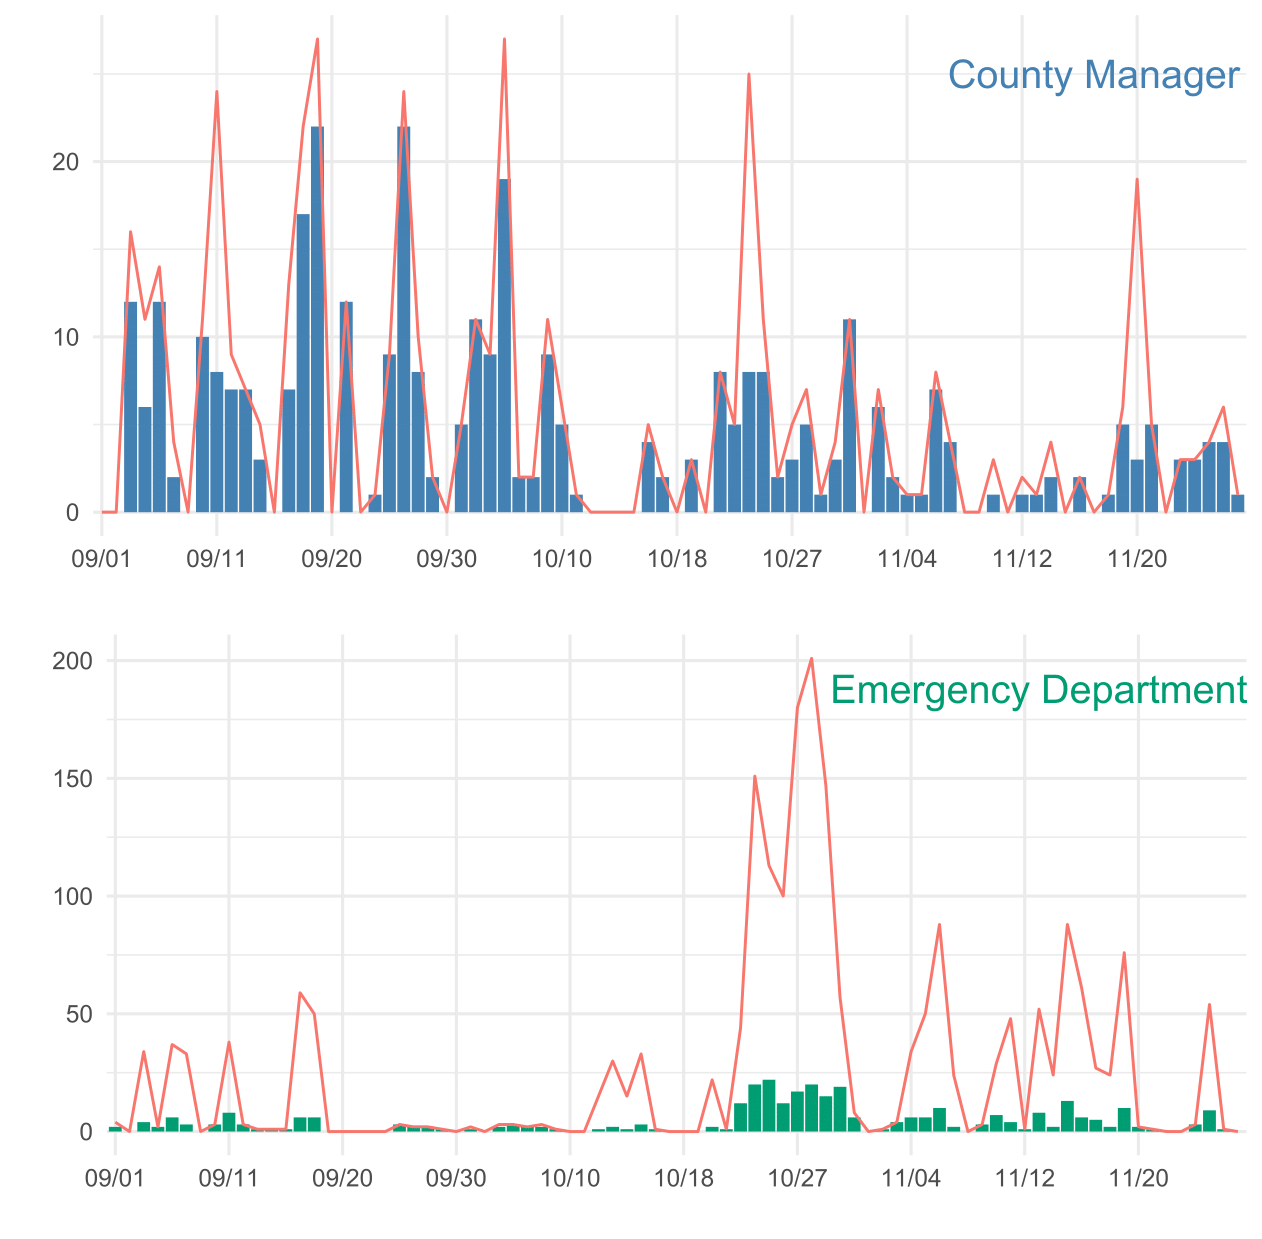
\includegraphics[width=.48\textwidth]{plots/EDAplot.png}  
	\caption{Sending behavior of two most active nodes in Dare County email data between 09/01/2012 and 11/30/2012. \textit{Top}: the number of emails per day sent by County manager (blue bar) and the number of recipients from this person per day (red line). \textit{Bottom}: the number of emails per day sent by emergency department official (green bar) and the number of recipients from this person per day (red line).}
\label{fig:EDAplot}
\vskip -0.15in
\end{figure}
\fi
\section{Interaction-partitioned Topic Model}\label{sec:model definition}

Data generated under the IPTM consists of $D$ unique documents. A single document, indexed by $d \in [D]$, is represented by the four components: the author $a_d \in [A]$, an indicator vector of recipients $\boldsymbol{r}_d = \{u_{dr} \}_{r=1}^{A}$, the timestamp $t_d \in (0, \infty)$, and a set of tokens $\boldsymbol{w}_d= \{w_{dn} \}_{n=1}^{N_d}$ that comprise the text of the document, where $N_d$ denotes the total number of tokens in a document. For simplicity, we assume that documents are ordered by time such that $t_d < t_{d+1}$.

\subsection{Interaction Patterns}\label{subsec:Interaction patterns}
They key idea that combines the IPTM component modeling ``what" with
the component modeling ``who," ``whom," and ``when" is that different
topics are associated with different interaction patterns.  Each interaction pattern $c \in [C]$ is characterized by a set of dynamic network features---such as the number of messages sent from $a$ to $r$ in some time interval---and corresponding coefficients. We associate each topic with the interaction pattern that best describes how people interact when talking about that topic. 
\textcolor{red}{
We first model each topic $k \in [K]$ as a dicrete distribution over $C$ unique interaction patterns,
\begin{equation}
	\boldsymbol{\psi}_k\sim \mbox{Dirichlet}\Big(\gamma, (\frac{1}{C},\ldots,\frac{1}{C})\Big),
\end{equation}
where $\gamma$ is the concentration parameter. Then, each topic-interaction pattern assignment $l_k$ is drawn from the 
\begin{equation}
l_k\sim \mbox{Multinomial}(\boldsymbol{\psi}_k),
\end{equation}
}
\subsection{Content Generating Process}\label{subsec:Content generating process}

The words $\boldsymbol{w}_d$ are generated according to latent Dirichlet allocation (LDA) \cite{Blei2003}, where we generate the corpus-wide global variables that describe the content via topics. As in LDA, we model each topic $k\in [K]$ as a discrete distribution over $V$ unique word types 
\begin{equation}
\boldsymbol{\phi}_k \sim \mbox{Dirichlet}\Big(\beta, (\frac{1}{V},\ldots,\frac{1}{V})\Big),
\end{equation}
where $\beta$ is the concentration parameter. Next, we assume a document- topic distribution over $K$ topics\\
\begin{equation}
\boldsymbol{\theta}_d \sim \mbox{Dirichlet}(\alpha, \boldsymbol{m}),
\end{equation}
where $\alpha$ is the concentration parameter and $\boldsymbol{m}=(m_1,\ldots,m_K)$ is the probability vector. Given that $\bar N_d = \max(1, N_d)$ where $N_d$ is known, a topic $z_{dn}$ is drawn from the document-topic distribution and then a word $w_{dn}$ is drawn from the chosen topic for each $n \in [\bar N_d]$---i.e.,
\begin{equation}
\begin{aligned}
&z_{dn} \sim \mbox{Multinomial}(\boldsymbol{\theta}_d),\\
&w_{dn} \sim\mbox{Multinomial} (\phi_{z_{dn}}).
\end{aligned}
\end{equation}

\textcolor{red}{\subsection{Additiaonl Derivation}}\label{subsec: Multinomial}
Then, the probability that a token is assigned to a topic corresponding to interaction pattern $c$ is
\begin{equation}
P(z_{dn}=k \cap l_k = c) = \sum_{k:l_k=c}{\theta}_{dk}\psi_{kc},
\end{equation}
and thus we can derive 
\begin{equation}
\begin{aligned}
&\bar N_{dc} \sim \mbox{Multinomial}(\bar N_{d} , \sum_{k:l_k=c}{\theta}_{dk}\psi_{kc}),\\
\end{aligned}
\end{equation}
where $\bar N_{dc}$ is the number of words in document $d$ that are assigned to topics corresponding to interaction pattern $c$. Using this property, we can define the expecation of proportions $E(\frac{\bar N_{dc} }{\bar N_{d}})=\frac{1}{\bar N_{d}}E(\bar N_{dc} )=\sum_{k:l_k=c}{\theta}_{dk}\psi_{kc}$ used for network statistics as $\pi_{dc}$ given the current value of $\theta$ and $\psi$
\begin{equation}
\pi_{dc}= \sum_{k:l_k=c}{\theta}_{dk}\psi_{kc},
\end{equation}
where we should infer $\theta$ and $\psi$ instead of integrating them out.
For network statistics, we replace $\frac{\bar N_{dc} }{\bar N_{dc}}$ by current estimate of $\pi_{dc}$.

\subsection{Tie Generating Process}\label{subsec:Tie generating process}
We generate ties---author $a_d$, recipients $\boldsymbol{r}_d$, and timestamp $t_d$---using a continuous-time process
that depends on the interaction patterns' various features. Conditioned on the content (Section \ref{subsec:Content generating process}), we assume the following steps of tie generating process. Much like in the SAOM \cite{snijders2010introduction}, we conceptualize tie generation as a process that is governed by senders acting in continuous time. 

\subsubsection{Latent Recipients}\label{subsubsec:Hypothetical Recipients}
For every possible author--recipient pair $(a,r)_{a \neq r}$, we define the ``interaction-pattern-specific recipient intensity":
\begin{equation}
\nu_{adrc} = {\boldsymbol{b}_c}^{\top}\boldsymbol{x}_{adrc},
\end{equation}
where $\boldsymbol{b}_c$ is $P$--dimensional vector of coefficients and $\boldsymbol{x}_{adrc}$ is a set of network features which vary depending on the hypotheses regarding canonical processes relevant to network theory such as popularity, reciprocity, and transitivity. We place a Normal prior $\boldsymbol{b}_c \sim N(\boldsymbol{\mu}_b, \Sigma_b)$.

In the example of email networks, we form the covariate vector for recipients $\boldsymbol{x}_{adrc}$ using dynamic network statistics focused on three time intervals prior to $t^+_{d-1}$ (i.e., immediately after the previous document was sent). We compute eight network statistics within each time interval \cite{PerryWolfe2012}, where the three time intervals are $[t^+_{d-1}-384h, t^+_{d-1}-96h), [t^+_{d-1}-96h, t^+_{d-1}-24h)$ and $[t^+_{d-1}-24h, t^+_{d-1})$. We define the intervals to have equal length in the log-scale, and use $i=1$ to denote the earliest interval---i.e., $[t^+_{d-1}-384h, t^+_{d-1}-96h)$---and i = 3 to denote the latest. The network statistics (illustrated in Figure \ref{fig:dynamic network statistics}) are:
\begin{figure}[b]
	\vskip -0.1in
	\centering
	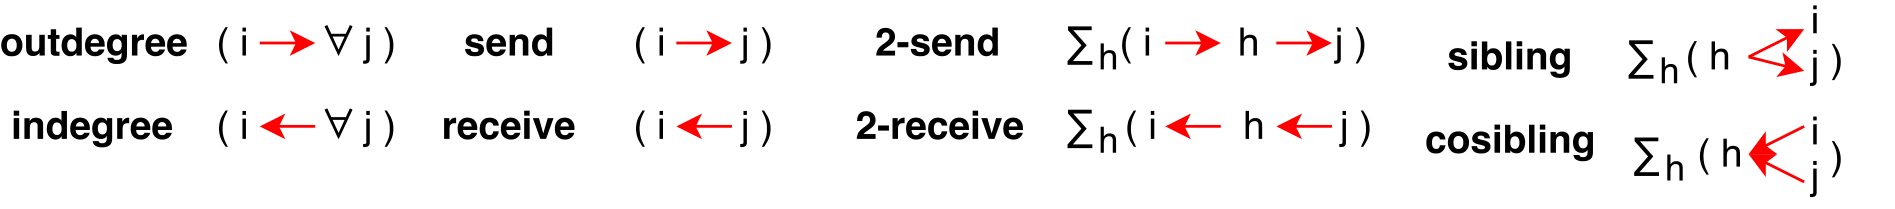
\includegraphics[height= 1.5cm, trim= 0cm 0cm 37cm 0cm, clip=true]{plots/netstats-1.png} \vspace{-.1cm}
	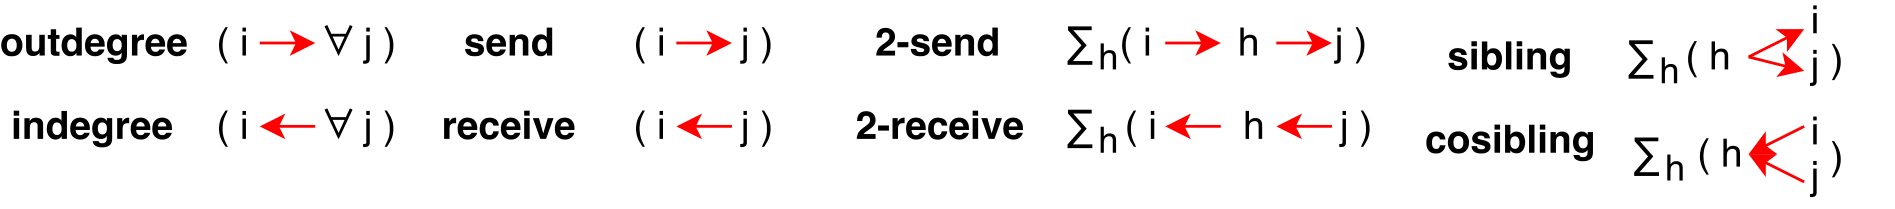
\includegraphics[height=1.5cm,, trim= 30cm 0cm 0cm 0cm, clip=true]{plots/netstats-1.png}
	\caption{Eight dynamic network statistics used for the application to email networks.}
	\label{fig:dynamic network statistics}	
\end{figure}
\begin{itemize}
	\item[1.] outdegree$(a,c,i)=\sum\limits_{d^\prime:t_{d^\prime \in i}} \textcolor{red}{\pi_{dc}}\delta(a_{d^\prime} = a)$.
	\item[2.] indegree$(r,c,i)=\sum\limits_{d^\prime:t_{d^\prime \in i}} \textcolor{red}{\pi_{dc}}\delta(u_{d^\prime r} = 1)$.
	\item[3.] send$(a,r,c,i)=\sum\limits_{d^\prime:t_{d^\prime \in i}} \textcolor{red}{\pi_{dc}}\delta(a_{d^\prime} = a)\delta(u_{d^\prime r} = 1)$.
	\item[4.] receive$(a,r,c,i)=\mbox{send}(r,a,c,i)$.
	\item[5.] 2-send$(a,r,c,i) $\\= $\sum\limits_{\substack{i^\prime, i^{\prime\prime}\geq i:\\i^\prime = i \mbox{ \small or }i^{\prime\prime}=i}}\sum\limits_{h \neq a, r} \mbox{send}(a,h,c,i^\prime)\mbox{send}(h,r,c,i^{\prime\prime})$.
	\item[6.] 2-receive$(a,r,c,i) $\\= $\sum\limits_{\substack{i^\prime, i^{\prime\prime}\geq i:\\i^\prime = i \mbox{ \small or }i^{\prime\prime}=i}}\sum\limits_{h \neq a, r} \mbox{send}(h,a,c,i^\prime)\mbox{send}(r,h,c,i^{\prime\prime})$.
	\item[6.] sibling$(a,r,c,i) $\\= $\sum\limits_{\substack{i^\prime, i^{\prime\prime}\geq i:\\i^\prime = i \mbox{ \small or }i^{\prime\prime}=i}}\sum\limits_{h \neq a, r} \mbox{send}(h,a,c,i^\prime)\mbox{send}(h,r,c,i^{\prime\prime})$.
	\item[6.] cosibling$(a,r,c,i) $\\= $\sum\limits_{\substack{i^\prime, i^{\prime\prime}\geq i:\\i^\prime = i \mbox{ \small or }i^{\prime\prime}=i}}\sum\limits_{h \neq a, r} \mbox{send}(a,h,c,i^\prime)\mbox{send}(r,h,c,i^{\prime\prime})$.
\end{itemize}
Note that in order to obtain two-path statistics (i.e., 2-send, 2-receive, sibling, and cosibling) within a single time interval $i$, we compute the number of two-paths from $a$ to $r$ in interaction pattern $c$ by summing over the pairs of intervals $(i^\prime, i^{\prime\prime})$ where the earlier email in the path was sent during interval $i$. 

We then compute the weighted average of $\{\nu_{adrc}\}_{c=1}^C$ and obtain the ``recipient intensity"---the likelihood of document $d$ being sent from $a$ to $r$--- using the the document's distribution over interaction patterns as mixture weights:
\begin{equation}
\lambda_{adr} =\sum_{c=1}^{C} \textcolor{red}{\pi_{dc}}\nu_{adrc},
\end{equation}
where $N_{dc}$ is the number of tokens assigned to topic $\{k:l_k=c\}$ in document $d$. 

Next, we hypothesize ``If $a$ were the
author of document $d$, who would be the recipent/recipients?" To do this, we draw each author's set of recipients from a non-empty Gibbs measure \cite{fellows2017removing}---a probability measure we defined in order to 1) allow multiple recipients or ``multicast", 2) prevent from obtaining zero recipient, and 3) ensure tractable normalizing constant. 

Because the IPTM allows multicast, we draw a binary (0/1) vector $\boldsymbol{u}_{ad}= (u_{ad1},
\ldots, u_{adA})$
\begin{equation} \boldsymbol{u}_{ad}  \sim
\mbox{Gibbs}(\delta, \boldsymbol{\lambda}_{ad}),
\end{equation}
where $\delta$ is a real number controlling the average number of recipients and $\boldsymbol{\lambda}_{id}= \{\lambda_{adr}\}_{r=1}^A$. We place a Normal prior $\delta \sim N(\mu_\delta,\sigma^2_\delta)$. In particular, we define $\mbox{Gibbs}(\delta, \boldsymbol{\lambda}_{ad})$ as
\begin{equation}
\begin{aligned}
&p(\boldsymbol{u}_{ad}|\delta, \boldsymbol{\lambda}_{ad}) \\&= \frac{\exp\Big\{\mbox{log}\big(\text{I}( \lVert \boldsymbol{u}_{ad}\rVert_1 > 0 )\big) + \sum_{r\neq a} (\delta+\lambda_{adr})u_{adr}\Big\}}{Z(\delta,\boldsymbol{\lambda}_{ad})} ,
\end{aligned}
\label{eqn:Gibbs}
\end{equation}
where $Z(\delta,\boldsymbol{\lambda}_{ad})= \prod_{r \neq a} (\mbox{exp}\{\delta+\lambda_{adr}\} + 1)-1$ is the normalizing constant and $\lVert \cdot \rVert_1$ is the $l_1$--norm. We provide the derivation of the normalizing constant as a tractable form in the supplementary material. 

\subsubsection{Latent Timestamps}\label{subsubsec:Hypothetical Timestamps}
Similarly, we hypothesize ``If $a$ were the author of document $d$, when would it be sent?" and define the ``interaction-pattern-specific timing rate"
\begin{equation}
\xi_{adc} = \boldsymbol{\eta}_c^\top \boldsymbol{y}_{adc},
\end{equation}
where $\boldsymbol{\eta}_c$ is $Q$--dimensional vector of coefficients with a Normal prior $\boldsymbol{\eta}_c \sim N(\boldsymbol{\mu}_\eta,\Sigma_\eta)$, and $\boldsymbol{y}_{adc}$ is a set of time-related covariates, which can be any feature that could affect timestamps of the document. 

For example, the covariate vector for timestamps $\boldsymbol{y}_{adc}$ can include author-specific intercepts to account for individual differences in document-sending behavior. In addition, some temporal features which possibly affect ``when to send" can be added---e.g., an indicator of weekends/weekdays and an indicator of AM/PM when the previous document was sent. 

Next, the ``timing rate" for author $i$ is then computed from the weighted average of $\{\xi_{adc}\}_{c=1}^C$ 
\begin{equation}
\mu_{ad} = \sum_{c=1}^C \textcolor{red}{\pi_{dc}}g^{-1}(\xi_{adc}),
\end{equation}
where $g(\cdot)$ is the appropriate link function such as identity, log, or inverse. 

In modeling ``when", we do not directly model the timestamp $t_d$. Instead, we assume that each author's the time-increment or ``time to next document" (i.e., $\tau_{d} = t_d-t_{d-1}$) is drawn from a specific distribution in the exponential family.  We follow the generalized linear model framework:
\begin{equation}
\begin{aligned}
E(\tau_{ad}) &= \mu_{ad},\\
V(\tau_{ad}) &= V(\mu_{ad}),
\end{aligned}
\end{equation}
where $\tau_{ad}$ is a positive real number. Possible choices of distribution include Exponential, Weibull, Gamma, and lognormal\footnote{lognormal distribution is not exponential family but can be used via modeling of $\log(\tau_d)$.} distributions, which are commonly used in time-to-event modeling. Based on the choice of distribution, we may introduce any additional parameter (e.g., $\sigma_\tau^2$) to account for the variance.

Our preliminary analysis revealed that the Dare County email networks and the Enron data set showed the best fitting when we assume lognormal distribution on the observed time-increments---i.e., $\log(\tau_{a_dd}) \sim N(\mu_{a_d d}, \sigma^2_\tau)$---compared to Gamma or Weibull distributions. We also observed significant lack-of-fit for single parameter distribution (e.g., Exponential distribution) since it failed to capture the variance in time-increments. Therefore, we chose lognormal distribution by taking the log-transformation and apply $\mu = E(\log(\tau_{ad})) = \mu_{ad}$ and $ \sigma_\tau^2=V(\log(\tau_{ad})) = V(\mu_{ad})$, using identity link function $g = I$.. 
\subsubsection{Actual Data}\label{subsubsec:Actual Data}
Finally, we choose the actual author, recipients, and timestamp---which will be observed---by selecting the author--recipient-set pair with the smallest time-increment \cite{snijders1996stochastic,snijders2017stochastic}:
\begin{equation}
\begin{aligned}
a_d &= \mbox{argmin}_{a}(\tau_{ad}),\\
\boldsymbol{r}_d &= \boldsymbol{u}_{a_d d},\\
t_d &=t_{d-1} + \tau_{a_d d}.
\end{aligned}
\end{equation}
Therefore, it is an author-driven process in that the author of a document determines its recipients and its timestamp, based on the author's urgency to send the document to chosen recipients. 

\textcolor{red}{\section{Posterior Inference}}\label{sec:Inference}
Now, the big joint distribution becomes
\begin{equation}
	\begin{aligned}
		&P(\boldsymbol{z},\boldsymbol{l},\boldsymbol{\theta}, \boldsymbol{\psi}, \boldsymbol{b},\boldsymbol{\eta}, \delta, \boldsymbol{u}, \boldsymbol{w}, \boldsymbol{a}, \boldsymbol{r}, \boldsymbol{t}| \gamma, \alpha, \beta, \boldsymbol{m},\boldsymbol{\mu}_b, \Sigma_b,\mu_\delta,\sigma^2_\delta)
		\\&\propto P(\boldsymbol{\theta}|\alpha, \boldsymbol{m})P(\boldsymbol{z}|\boldsymbol{\theta})P(\boldsymbol{w}|\boldsymbol{z})
		 P(\boldsymbol{\psi}|\gamma) P(\boldsymbol{l}|\boldsymbol{\psi})\\&\times P(\boldsymbol{b}|\boldsymbol{\mu}_b, \Sigma_b ) P(\boldsymbol{\eta}|\boldsymbol{\mu}_\eta, \Sigma_\eta )
		 P(\delta|\mu_\delta,\sigma^2_\delta) P(\boldsymbol{u}|\boldsymbol{\theta},\boldsymbol{\psi}, \boldsymbol{l},\boldsymbol{b}, \delta)\\&\times P(\boldsymbol{a}, \boldsymbol{t}|\boldsymbol{\theta},\boldsymbol{\psi},\boldsymbol{l}, \boldsymbol{\eta})P(\boldsymbol{r}|\boldsymbol{a},\boldsymbol{u}),
	\end{aligned}
\end{equation}
and here we will sequentially update $\boldsymbol{z},\boldsymbol{l},\boldsymbol{\theta}, \boldsymbol{\psi}, \boldsymbol{b},\boldsymbol{\eta}, \delta, \boldsymbol{u}$.

Since we only integrate out $\boldsymbol{\phi}$ but let $\boldsymbol{\theta}$ not integrated, the conditional posterior for topic assignment $z_{dn}$ is then simple LDA with current estimate of $\boldsymbol{\theta}$:
\begin{equation}
\begin{aligned}
&p(z_{dn}=k| \boldsymbol{z}_{\backslash dn}, \boldsymbol{\theta}, \boldsymbol{\psi}, \boldsymbol{l}, \boldsymbol{b},\boldsymbol{\eta}, \delta, \boldsymbol{u}, \boldsymbol{w}, \boldsymbol{a}, \boldsymbol{r}, \boldsymbol{t}, \alpha, \beta, \boldsymbol{m})\\&\propto P(z_{dn}=k|\boldsymbol{\theta}_d)\times P(w_{dn}=w|z_{dn}=k, \boldsymbol{z}_{\backslash dn}, \boldsymbol{w}, \beta)
\\&\propto 
\theta_{dk} \times 	  \frac{N_{w_{dn}k, \backslash dn}+\frac{\beta}{V}}{N_{k, \backslash dn}+\beta},
\end{aligned}
\end{equation}
where the subscript $\backslash dn$ denote the exclusion of document $d$ and $n^{th}$ element in document $d$, and $N_{w_{dn}k, \backslash dn}$ is the number of tokens assigned to topic $k$ whose type is the same as that of $w_{dn}$, excluding $w_{dn}$ itself. 

We now add two steps for each outer iterations--- updates on $\boldsymbol{\theta}$ and $\boldsymbol{\psi}$. For $d \in [D]$, we update the document-topic distribution as below:
\begin{equation}
\begin{aligned}
&P(\boldsymbol{\theta}_{d}|z_d, \alpha, \boldsymbol{m},  \boldsymbol{u},  \boldsymbol{a},  \boldsymbol{t}) \\&\propto P(\boldsymbol{z}|\boldsymbol{\theta}_d)P(\boldsymbol{\theta}_d|\alpha, \boldsymbol{m})P(\boldsymbol{u}|\boldsymbol{\theta},\boldsymbol{\psi},\boldsymbol{l}, \boldsymbol{b}, \delta)P(\boldsymbol{a}, \boldsymbol{t}|\boldsymbol{\theta},\boldsymbol{\psi}, \boldsymbol{l},\boldsymbol{\eta})
\\&\propto \Big(\prod_{n=1}^{\bar N_d} P(z_{dn}|\boldsymbol{\theta}_{d}) P(\boldsymbol{\theta}_{d}|\alpha, \boldsymbol{m})\Big)\\&\times \Big(\prod_{d=d+1}^{d^*}P(\boldsymbol{u}_d|\boldsymbol{\theta},\boldsymbol{\psi}, \boldsymbol{b}, \delta)\Big)\times \Big(P(\boldsymbol{a}_d, \boldsymbol{t}_d|\boldsymbol{\theta},\boldsymbol{\psi}, \boldsymbol{\eta})\Big)\\
&\propto\Big(\prod_{n=1}^{\bar N_d} \theta_{dz_{dn}}\times \prod_{k=1}^{K} \theta_{dk}^{\alpha m_k - 1}\Big)\\&\times\Big(\prod_{d=d+1}^{d^*}\Big(
\prod_{a=1}^A \frac{\exp\Big\{\mbox{log}\big(\text{I}( \lVert \boldsymbol{u}_{ad}\rVert_1 > 0)\big) + \sum\limits_{r \neq a} (\delta+\lambda_{adr})u_{adr}\Big\}}{Z(\delta,\boldsymbol{\lambda}_{ad})}\Big)\Big)
\\&\times\Big(\varphi_{\tau}(\tau_{d}; \mu_{a_d d}, \sigma_\tau^2)\times \prod_{a\neq a_d}\big(1-\Phi_{\tau}(\tau_{d}; \mu_{a d}, \sigma_\tau^2) \big)\Big)\\
&\propto\Big(\prod_{k=1}^{K} \theta_{dk}^{\bar N_{dk}+\alpha m_k - 1}\Big)\\&\times\Big(\prod_{d=d+1}^{d^*}\Big(
\prod_{a=1}^A \frac{\exp\Big\{\mbox{log}\big(\text{I}( \lVert \boldsymbol{u}_{ad}\rVert_1 > 0)\big) + \sum\limits_{r \neq a} (\delta+\lambda_{adr})u_{adr}\Big\}}{Z(\delta,\boldsymbol{\lambda}_{ad})}\Big)\Big)
\\&\times\Big(\varphi_{\tau}(\tau_{d}; \mu_{a_d d}, \sigma_\tau^2)\times \prod_{a\neq a_d}\big(1-\Phi_{\tau}(\tau_{d}; \mu_{a d}, \sigma_\tau^2) \big)\Big)\\
& \nsim \mbox{Dirichlet}(\bar N_{d1} + \alpha m_1,\ldots, \bar N_{dK} + \alpha m_K),
\end{aligned}
\end{equation}
and for $k \in [K]$, we update the topic-interaction pattern distribution using 
\begin{equation}
\begin{aligned}
&P(\boldsymbol{\psi}_{k}|\boldsymbol{l},  \gamma,\boldsymbol{u},  \boldsymbol{a},  \boldsymbol{t})
\\&\propto P(\boldsymbol{\psi}|\gamma)P(\boldsymbol{l}|\boldsymbol{\psi})P(\boldsymbol{u}|\boldsymbol{\theta},\boldsymbol{\psi},\boldsymbol{l}, \boldsymbol{b}, \delta)P(\boldsymbol{a}, \boldsymbol{t}|\boldsymbol{\theta},\boldsymbol{\psi}, \boldsymbol{l},\boldsymbol{\eta})
\\&\propto\Big(\prod_{c=1}^{C} \psi_{kc}^{N_{kc}+\gamma/C - 1}\Big)\\&\times\Big(\prod_{d=d+1}^{d^*}\Big(
\prod_{a=1}^A \frac{\exp\Big\{\mbox{log}\big(\text{I}( \lVert \boldsymbol{u}_{ad}\rVert_1 > 0)\big) + \sum\limits_{r \neq a} (\delta+\lambda_{adr})u_{adr}\Big\}}{Z(\delta,\boldsymbol{\lambda}_{ad})}\Big)\Big)
\\&\times\Big(\varphi_{\tau}(\tau_{d}; \mu_{a_d d}, \sigma_\tau^2)\times \prod_{a\neq a_d}\big(1-\Phi_{\tau}(\tau_{d}; \mu_{a d}, \sigma_\tau^2) \big)\Big)\\
& \nsim  \mbox{Dirichlet}(N_{k1}+ \gamma/C,\ldots, N_{kC} + \gamma/C),
\end{aligned}
\end{equation}
where $N_{kc}$ is the number of topics assigned to interaction pattern $c$.

\textcolor{red}{After these two parameters $\boldsymbol{\theta}$ and $\boldsymbol{\psi}$ are updated (i.e. $\pi_{dc}$), we recalculate the network statistics $x_{adrc}$, $\lambda_{adr}$ and $\xi_{adc}$ once and use it for the rest of updates. However, they both require Metropolis-Hastings (or something else similar). Is it worth trying? I don't think so...}

% Acknowledgements should only appear in the accepted version.

\iffalse

% In the unusual situation where you want a paper to appear in the
% references without citing it in the main text, use \nocite
\nocite{langley00}

\bibliography{IPTM}
\bibliographystyle{icml2018}
		\fi
%%%%%%%%%%%%%%%%%%%%%%%%%%%%%%%%%%%%%%%%%%%%%%%%%%%%%%%%%%%%%%%%%%%%%%%%%%%%%%%
%%%%%%%%%%%%%%%%%%%%%%%%%%%%%%%%%%%%%%%%%%%%%%%%%%%%%%%%%%%%%%%%%%%%%%%%%%%%%%%
% DELETE THIS PART. DO NOT PLACE CONTENT AFTER THE REFERENCES!
%%%%%%%%%%%%%%%%%%%%%%%%%%%%%%%%%%%%%%%%%%%%%%%%%%%%%%%%%%%%%%%%%%%%%%%%%%%%%%%
%%%%%%%%%%%%%%%%%%%%%%%%%%%%%%%%%%%%%%%%%%%%%%%%%%%%%%%%%%%%%%%%%%%%%%%%%%%%%%%
%%%%%%%%%%%%%%%%%%%%%%%%%%%%%%%%%%%%%%%%%%%%%%%%%%%%%%%%%%%%%%%%%%%%%%%%%%%%%%%
%%%%%%%%%%%%%%%%%%%%%%%%%%%%%%%%%%%%%%%%%%%%%%%%%%%%%%%%%%%%%%%%%%%%%%%%%%%%%%%


\end{document}


% This document was modified from the file originally made available by
% Pat Langley and Andrea Danyluk for ICML-2K. This version was created
% by Iain Murray in 2018. It was modified from a version from Dan Roy in
% 2017, which was based on a version from Lise Getoor and Tobias
% Scheffer, which was slightly modified from the 2010 version by
% Thorsten Joachims & Johannes Fuernkranz, slightly modified from the
% 2009 version by Kiri Wagstaff and Sam Roweis's 2008 version, which is
% slightly modified from Prasad Tadepalli's 2007 version which is a
% lightly changed version of the previous year's version by Andrew
% Moore, which was in turn edited from those of Kristian Kersting and
% Codrina Lauth. Alex Smola contributed to the algorithmic style files.
